\section{Evaluation}
\label{evaluation}
During a comprehensive project like this, which has spanned five months, the group has learned a lot. This chapter will illustrate what went well, what did not go according to plan and what the group could have done different.

\subsection{Project evaluation}

This section will evaluate the overall group performance, as well as reflecting over the different problems that the group encountered during the project.

\subsubsection{Scrum}
\label{scrum_eval}
Using Scrum required a lot of effort and responsibility from each group member. There was times in the project period, especially in sprint 4-5, when some group members struggled with both effort and motivation. We got in the habit of delaying daily scrums until the evening, which some times resulted in forgetting them completely. This may have effected the group in a bad way because we sometimes lost track of what had been done from day to day.

The group acknowledged the urgency of taking immediate actions. This is where the risk analysis came in handy. The situation was remedied by not ignoring the issue in meetings, and reminding everyone how important it was to stay focused while working in a group. If one or more group members did not show up to work sessions, it was agreed upon that everyone were to do a write up of what was done that day. This is also why sprint retrospects were so important, because it forced everyone to think through what parts of the scrum we wanted to improve upon. 

After these actions were taken the sprints went better. Although some issues like work distribution, seemed to have a cascading effect on some group members. Because they at some point lost track, it was hard to keep up on both terminology and technology discussions. It is hard to point out exactly why this was the case, even though everyone in the group were aware of it happening. It might be a case of lack in motivation amongst some team members combined with the fact that we did not have a group leader: As mentioned in Project Planning, we thought it was important for an agile development team to be autonomous.

\subsubsection{Communication}
The group feels that the quality of communication has had its ups and downs. It is especially easy to get so focused on the current task one is working on, that one tends to forget to communicate to the group what is being worked on. A remedial action would be for the group to take a break and explain what each and everyone is doing. It is understandable that it can be difficult for the person who feels that he has lost his overview, to call for such a break.

One tactic to avoid this is to use tools like issue trackers like JIRA, so that group members do not have to ask all the time. Unfortunately, things got a little out of hand at times, and issues were not always recorded or estimated. Again, some of the fault for this might have resided in our research, as some tasks were virtually impossible to estimate. In retrospect, we are happy with the way we did manage to utilize JIRA, considering it being the first time we used the technology and way of working.

The risk assessment sheet said that when a group member falls ill the rest of the group must make up for his lost time. This was good in the sense that we did not fall behind, but it affected the group dynamic because the gap between the healthy group members and the ill ones grew.

Sprint retrospect meetings were a good way for the group to update all group members, and make them aware of such situations. These meetings also helped to remind everyone to keep communicating what they were doing, what they planned to do and what problems they had encountered.

The means of communication, next to the work sessions at campus, has been through Google Hangouts. The group feels that this has worked well. It has been a channel for group members to ask questions and get answers fairly quickly, and a good tool for quickly planning a meeting for the next day.

\subsubsection{Research and planning}
\label{researchEval}
The research period of the project ended up being really comprehensive. Several of our contacts suggested that what we were trying to accomplish was more of master or doctorate thesis, rather than a bachelor thesis. This might have had with our inability to restrict the project; at one point we wanted to solve all the compatibility problems existing between today's systems, at the same time as we tried to introduce infrastructure for multimedia storage at hospitals. This demonstrates both our commitment and dedication to the task, which again is reflected in our view on the project as a whole: We have had genuinely fun working with this project, and we are proud over the amount of knowledge we have gained.

As a consequence of how the research went, the sprint overview and goals, ended up looking somewhat different as was planned as shown in Figure \ref{fig:sprinter_oversikt_rev}. Sprint 3 ended up having no epics completed. During this sprint, in total two people were sick and another two was on leave on different occations. The parts of the application that was finished at that time did not complete any epics.

\begin{figure}[H]
\centering
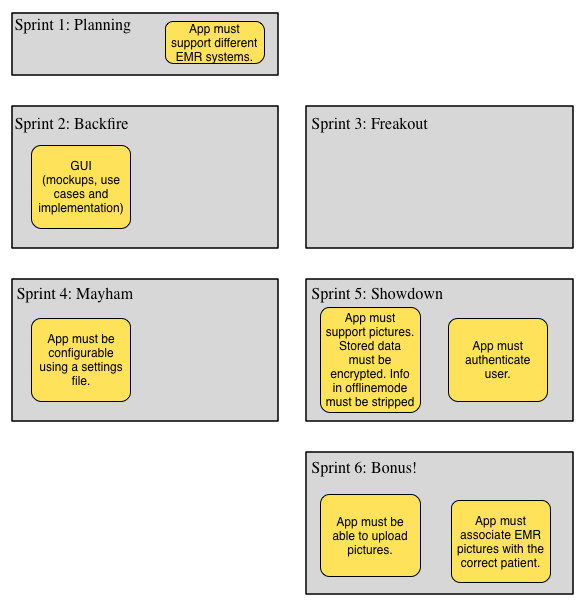
\includegraphics[scale=0.7]{img/sprint_overview_rev.png}
\caption{Revised overview of the sprints and their goals}
\label{fig:sprinter_oversikt_rev}
\end{figure}


\subsubsection{Work distribution}
The group has also discussed the situation of work distribution. During development, research, especially in regards to the hospital information systems, has mostly been done by two group members, and for a huge part of the development process only two other group members had control over the code. This was both good and bad. Because the research done in this area has not been traditional lexical research, having two people doing most of the research had it benefits. This type of research mostly consisted of email and phone calls. You tried to ask the correct questions to the correct people, and were pointed, sometimes, in several directions in their replies. By having two people doing this research, it was easier for them to follow the trail so to speak.

Thinking about the negative aspects of doing it this way we can name a few. It’s especially important for these two group members to communicate their findings to the rest of the group. And for the remaining group members to actively take an interested in how their research is going.

Having discussed the group’s problems in regards to daily scrum meetings, the group has become aware that this process of doing the research might not have been the best. Especially if one of these group members were to fall ill for a major part of the development.

As the rest of the group struggled to keep up with the research, development of the application itself was started, and the result was the same as with the research part. The two group members that started implementing became the two members that had written almost all the code written in the first sprints, making it hard for the other group members to get into and understand the code, as they were unfamiliar with the Android development platform to begin with.

With that said, the group feels that by dividing the work this way, a lot of time was saved by doing multiple tasks at once, and that the process of catching up afterwards took much less time than it would have taken to do one task at a time.

\newpage

\subsection{Product evaluation}
\label{productEval}

This section will evaluate the design choices of the Android application and explain what the group should have done different, what is missing and considerations the customer should take in regards to the future.

\subsubsection{Requirements not met}
The only requirement not met is offline mode. A discussion on this can be found in section \ref{evaloffline}.

\subsubsection{Settings}
The settings layout for the application was designed to hold data that specifies the service and authentication information. Although the application currently only supports LDAP/LDAPS, both the code and the settings layout is structured in such a way that other protocols can be implemented on a later stage. With this in mind, the customer is advised to consider whether to expand on the current code, so to support other authentication systems, or to scrape this solution, and move this functionality over to the service. The authentication architecture was researched and developed on an early stage of the development, whereas the service needed a lot more time and refinement before it was implemented. Since the service architecture change so dramatically from its first draft, it was never considered to bundle the authentication with the pre-existing tasks. If the application was to be released internationally, the consequences of the current solution would be that the application only works with hospitals information systems using with Active Directory. 


\subsubsection{User interface}
The user interface has been a priority throughout the project, as it was considered imperative to keep the flow of the application as simple and intuitive as possible. Although the group feels that the usability requirements are fulfilled, there are still some issues that should be addressed.

Throughout the application, feedback about system status should be better. This was not a priority during development process, and as a result of this, proper feedback is missing during certain actions. As of present, the "Login"-view only gives the user an unspecific error message if something went wrong during login (e.g. wrong credentials, error connection to authentication server). The "Settings"-view also lacks proper feedback, and does not notify the user if certain settings are missing or if the device is unable to connect to the server.

It is also worth noting that the interface was designed to be used in portrait mode only, and that the customer therefore should consider restricting the application to this view. It can also be considered to add support for landscape view. For instance, if the application is to be used on an Android tablet, this functionality would accommodate nicely.


\subsubsection{Offline mode}
\label{evaloffline}
Offline mode was a feature that was given a lot of thought during the initial phase of the project. Although it was not one of the primary features requested by the customer, it was still a finesse that would make the end product a lot more versatile in its usage. As mentioned in the implementation chapter, an early version of the application supported offline mode, but as the application development progressed this feature became more and more outdated. The final version of the application is therefore released without a fully functional offline mode. With that said, there is just minor changes needed to the application, to make offline mode work again. 

Currently, the application has no restrictions on letting the user upload images, or otherwise proceed with an examination after logging in. Should the session time out, or the device loose network connectivity, the only thing that happens is that sensitive data gets stripped from the user interface. Because offline mode required database access, and the final version of the database encryption design made logging in to the application necessary to use the database, the offline mode feature was discontinued.

As a result, a full refactoring of the offline mode functionality is recommended. Instead of stripping sensitive data during offline mode, the (already implemented) session system should be used. Although this restricts usage to users that have logged in at least once, it gives the great feature of full offline functionality. The doctor can log in as usual, and can conduct an examination. When the user arrives to the "Upload"-view, he should get the option of saving the examination, rather than uploading it.
This refactoring would require minor changes to the session system to support authenticating through checking database access when no network is available. For security reason, this would also require built-in brute-force detection.
The user should also be informed when the session has timed out or connection has been lost and get the option to log in again.

\subsubsection{Security}
Making sure the application satisfied the security requirements, was the most important aspect of this project. Before these requirements can be considered to be fulfilled, certain issues needs to be addressed. 

One of the most important issues is that the department credentials (as mentioned in section \ref{serviceDescription}) currently is stored in SharedPreferences. Although encrypted, this  solution is not considered a secure enough. Instead, these credentials should reside in each doctor’s encrypted database. Whereas the current application is designed to prompt the technical user for these credentials, the final version should prompt the doctor during first time login. 

Among other safety issues, proper deletion of images has not yet been implemented. In the current implementation, the application only receives the path of each image, and removes this path after upload. After images are uploaded, it is reasonable to assume that the images no longer serves any practical use to the user, and that they therefore should be deleted. 

Because of a bug, the application will currently not delete all data when the application is reconfigured. This should be considered as a major security threat, as a malicious service can replace the original without the users knowing.

The "Delete everything"-option in the settings menu is currently not password protected, which enable a malicious user to delete data. Although not a major security concern, this could still lead to loss of data not yet uploaded to the server. Of the bigger potential safety issues, the encryption library used with the database, SLQCipher, currently prints stack traces if the password attempted to decrypt the database with is wrong, caused when the authentication password is changed. See technical risk 1.4 in Appendix \ref{technicalrisks}.

To improve on the current security measures, the customer should also consider implementing brute force detection. Given that the offline mode functionality is refactored as described above, it would be possible to brute force user credentials while the application is offline.


\subsubsection{Service}
The service ended up being the biggest feature in the application. The interoperability that comes with the service implementation gives the application the potential to work with any hospital information system in the world. Whilst the application currently sends its messages using ArrayLists, the final product should rather depend on HashMaps. HashMaps is a lot more scalable, and are therefore easier to maintain. Using HashMaps renders the order of the data in messages irrelevant, whilst this order of the message is currently imperative if the message is to be interpreted correctly. 

In addition to refactoring the lists, the error message currently in use should also be assessed. The current error system is intended to send a Boolean value with the message, where the Boolean is dependent on the on the outcome of the operation (successful or not). If the Boolean is false, an error message is also attached. 

Since the application cannot vouch for the content of this message, the message system should be redesigned. An array of error codes should be designed, so that the service can return a known error to the application. Based on the error code, the application should display a relevant error to the user. 

In regards to the backup service developed during this project, this service should not be used during production. The license for the iText library (see section\ref{itextlib}) does not cover commercial use without purchasing the proper licence.

\subsubsection{Session}
The session feature was implemented to require that the user logged in only once during a given time interval. As described in section \ref{sessionimplement}, the session is also used to check network connectivity. To support the necessary changes to offline mode described in section \ref{evaloffline}, the validation and login methods should be changed to use the database to authenticate when no network is available.

\subsubsection{Application logic}
Some of the logic done in the application must be assessed if the application is to be released internationally. The patient's date of birth is currently based on the patient's SSN, which is not the case in many other countries (e.g. United States). The ID ascertained through the automatic scan is also assumed to be the patients SSN, which also is not the case in every other country. In many other systems this ID is an ID generated by PAS, which currently is not supported by the service system. 

A new examination should be created on start up, not in the examination view. Today, examination objects are created first when the examination activity starts, and examinations will therefore be overwritten if they do not reach this activity. 

\subsubsection{The code itself}
Time consuming or resource intensive tasks should run on their own thread. This is not yet implemented during automatic identification using the QR scanner, and should be addressed. In respect to the code we have produced, it should be reviewed in order to identify additional patterns and simplifications that would reduce the code complexity, give better performance as well as better re-use of code through polymorphic variants. Examples of code that should be reused is AlertDialogs for writing examination, and image comments as well as a dialog for logging in. How the application handles exceptions should also be reviewed. 

\subsubsection{Final release}
Before a final release, tests should be conducted, including unit testing and further security testing. As previously mentioned, the group does not consider itself qualified to test the application to the extent necessary to claim it to be safe for use.  

As of now, the application does not provide restrictions to which file types that can be sent to the service. This was intentionally left undone, as it was decided that this was a decision the customer should take. 

Since the application developed during this project was intended as a proof of concept, we were not reluctant in using open source libraries. Before a release, the customer should consider to implement their own functionality for both QR-scanning and image viewing, as well as getting a commercial license for the SQLCipher encryption library. 
A new feature the customer might also consider implementing, is functionality allowing the user to draw or annotate on to images on post examination. However, if this is to be considered, further research should be conducted in order to uncover if this is a feature the industry would benefit by having. With that said, the feedback the group has received when suggesting this feature for individuals in the industry, has been entirely positive.

Although not described during this report, the customer expressed desire to allow for the user to use voice recordings during the examination. This feature has not been worked on, but during development, Android's native speech-to-text feature has been tested while adding notes. This feature has worked exceptionally well when dictating in English, and is a technology the customer might want to look further into. 